\definecolor{singleShotColor}{RGB}{196,106,28}
\definecolor{pipelineColor}{RGB}{44,138,100}
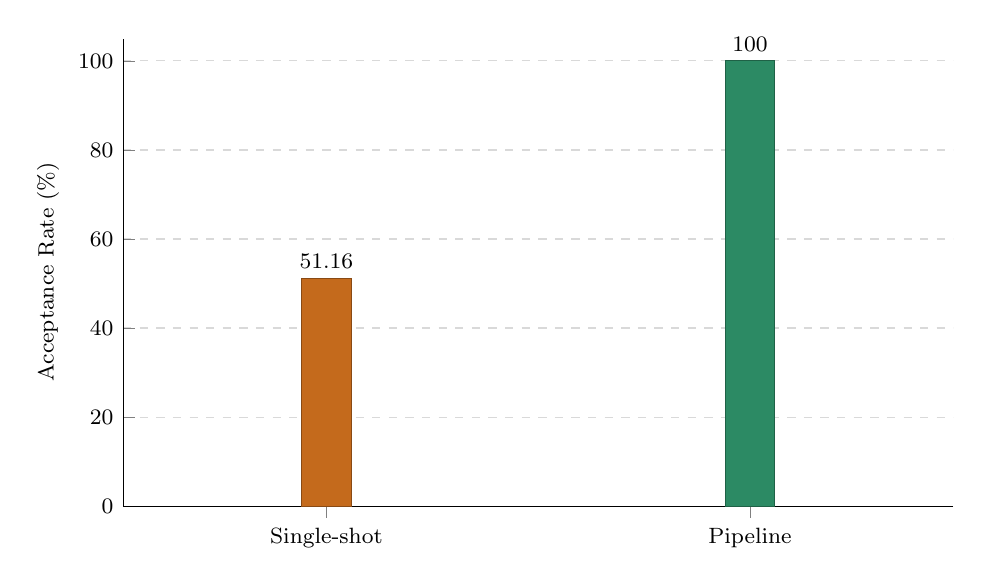
\begin{tikzpicture}
\begin{axis}[
    ybar,
    bar width=18pt,
    width=\columnwidth,
    height=0.62\columnwidth,
    ymin=0,
    ymax=105,
    ylabel={Acceptance Rate (\%)},
    symbolic x coords={Single-shot,Pipeline},
    xtick={Single-shot,Pipeline},
    xticklabels={Single-shot,Pipeline},
    nodes near coords,
    nodes near coords align={vertical},
    nodes near coords style={font=\footnotesize,text=black},
    enlarge x limits=0.48,
    axis lines*=left,
    ymajorgrids=true,
    grid style={dashed,gray!30},
    tick label style={font=\footnotesize},
    label style={font=\footnotesize},
]
\addplot+[bar shift=0pt, fill=singleShotColor, draw=singleShotColor!70!black] coordinates {
    (Single-shot,51.16)
};
\addplot+[bar shift=0pt, fill=pipelineColor, draw=pipelineColor!70!black] coordinates {
    (Pipeline,100.00)
};
\end{axis}
\end{tikzpicture}
